\section{Testing}
I am going to hand compile and trace a series of programs to validate that the system is functioning correctly, as well as demonistrating various error messages the compiler can produce should it encounter syntax errors within the source code. I will also demonstrate how the graphical display and debugger for the virtual machine work - showing the robustness and performance of the system by compiling and executing a game of pong. Below is the link to the testing video:

https://www.youtube.com/watch?v=KQ6ibE77F8w

\subsection{Testing Table}

\begin{longtable}{|p{1cm}|p{5cm}|p{5cm}|p{2cm}|} 
    \hline
        No & Test & Purpose & Timestamp \\ 
    \hline
        1.1
        & 
        Assemble a program that counts to 15. 
        &
        To ensure the assembler correctly assembles programs into machine code.
        & 
        10:53-14:30
        \\
    \hline
        1.2
        & 
        Assemble a program containing branch and jump instructions between labels.
        &
        To ensure jump instructions calculate absolute addresses, and branch instructions calculate relative offsets. Validates that the assembler can correctly use the position of labels within the source code to determine these values.
        & 
        14:30-16:26
        \\
    \hline
        1.3
        & 
        Assemble a program containing macro instructions.
        &
        To ensure that the assembler can correctly expand and assemble macro instructions by validating the number of instructions produced and their opcodes.
        & 
        16:26-18:33
        \\
    \hline
        1.4
        & 
        Attempt to assemble a program containing an invalid character.
        &
        To ensure the assembler halts compilation and throws a syntax error, pointing out the position of the invalid character in source code.
        & 
        18:47-19:12
        \\
    \hline
        1.5
        & 
        Attempt to assemble a program containing a undefined mnuemonic.
        &
        To ensure the assembler halts compilation and throws a syntax error, specifying that the mneumonic encountered is not defined within the instruction set.
        & 
        19:18-19:30
        \\
    \hline
        1.6
        & 
        Attempt to assemble a program containing an overflowinging integer.
        &
        To ensure the assembler throws an error specifying that the number it is attempting to assemble is too large to fit in 16 bits. 
        & 
        19:30-19:40
        \\
    \hline
        1.7
        & 
        Attempt to assemble a program containing an unexpected register or invalid label.
        &
        To ensure the assembler throws an error specifying that the label hasn't been defined within the program, or that the register doesn't exist. 
        & 
        19:40-20:15
        \\
    \hline
        2.1
        & 
        Trace the execution of a program to count to 15.
        &
        Ensure the computer exhibits the correct state and control flow when executing a binary executable. 
        & 
        21:10-22:20
        \\
    \hline
        2.2
        & 
        Trace the execution of a program containing jump and branch instructions.
        &
        Validates whether the virtual machine can correctly jump between instructions and follow the control flow specified within the program.
        & 
        22:20-24:14
        \\
    \hline
        2.3
        & 
        Trace the execution of a program to calculate the factorial of a number.
        &
        An integration test for the assembler and virtual machine together in order to assemble and execute a more complex program involving the stack and subroutines. 
        & 
        24:15-26:47
        \\
    \hline
        2.4
        & 
        Test the graphical display by executing programs that involve writing piexls to the screen.
        &
        Ensures the state of pixels on the screen directly correspond to the state of VRAM. Validates that writing to the screen via offsets, and within a loop function as expected.
        & 
        26:47-30:35
        \\
    \hline
        3.1
        & 
        Write and compile a program in the high level langauge to calculate the factorial of a number.
        & 
        Demonstrate that the assembly code produced, after being copiled and executed - correctly exhibits the functionality of the high level program.
        & 
        31:50-34:17
        \\
    \hline
        3.2
        & 
        Attempt to compile a program containing an unexpected keyword.
        &
        Validate that the compiler halts compilation and throws a syntax error pointing out the location of the error, and suggesting alternative keywords to fix the issue. 
        & 
        32:15-32:35
        \\
    \hline
        3.3
        & 
        Attempt to compile a program without a main subroutine
        &
        Validate that the linker throws an error when attempting to compile a program without an entry point. 
        & 
        32:30-32:38
        \\
    \hline
        3.4
        & 
        Attempt to compile a program attempting to assign a value of the incorrect type to a variable.
        &
        Ensure that the compiler throws a type error and halts compilation. 
        & 
        32:50-32:58
        \\
    \hline
        3.5
        & 
        Compile and execute a program that uses VRAM and the graphical display to demonstrate passing by value and reference within my language. 
        &
        Demonstrate how dereferencing pointers to variables can be used within a subroutine to modify 'external' variables, and how to write to memory by dereferencing a memory location including using pointer aithmetic for offsets. 
        & 
        34:22-36:36
        \\
    \hline
        3.6
        & 
        Attempt to compile a program containing a reference to an undeclared subroutine.
        &
        Ensure that the compiler halts compilation and points to the location of the undeclared subroutine in the source code.
        & 
        36:36-36:47
        \\
    \hline
        3.7
        & 
        Compile and exeute a program that demonstrates pointer arithmetic. 
        &   
        Validates pointer arithmetic, dereferencing and memory addresses all function correclty within the langauge. Including that dereferencing a variable declared as a pointer to another variable, who's since had its contents changed - should, when dereferenced - also exhibit that new value. 
        & 
        36:48-38:48
        \\
    \hline
        3.8
        & 
        Compile and exeute pong. 
        &   
        An integration test that demonstrates how all three components of the system can function together to compile a complex program that involves all elements of the langauge: subroutines, stack frames, constants, conditionals and loops, pointers and references, etc. And furthermore how the CPU can use a delay timer to create a game playable in real time that interfaces with a keyboard. Ensuring the system is sufficiently optimised to execute at 60 frames per second. 
        & 
        38:38-41:50
        \\
    \hline
\end{longtable} 

\subsection{Testing Key Algorithms}

\subsubsection{Parsing}
I will run a series of tests against the key algorithms of the project in order to ensure the code works as intended. Starting with the Parser. This will ensure that each type of program statement is parsed into the correct nodes, and the system throws the expected errors when it encounters invalid syntax. Each test case includes the code being parsed, followed by the output of the lexer and parser respectively, along with any error messages.

\begin{longtable}{|p{12cm}|p{4cm}|} 
    \hline
        Program & Result \\ 
    \hline
        \raisebox{-\totalheight}{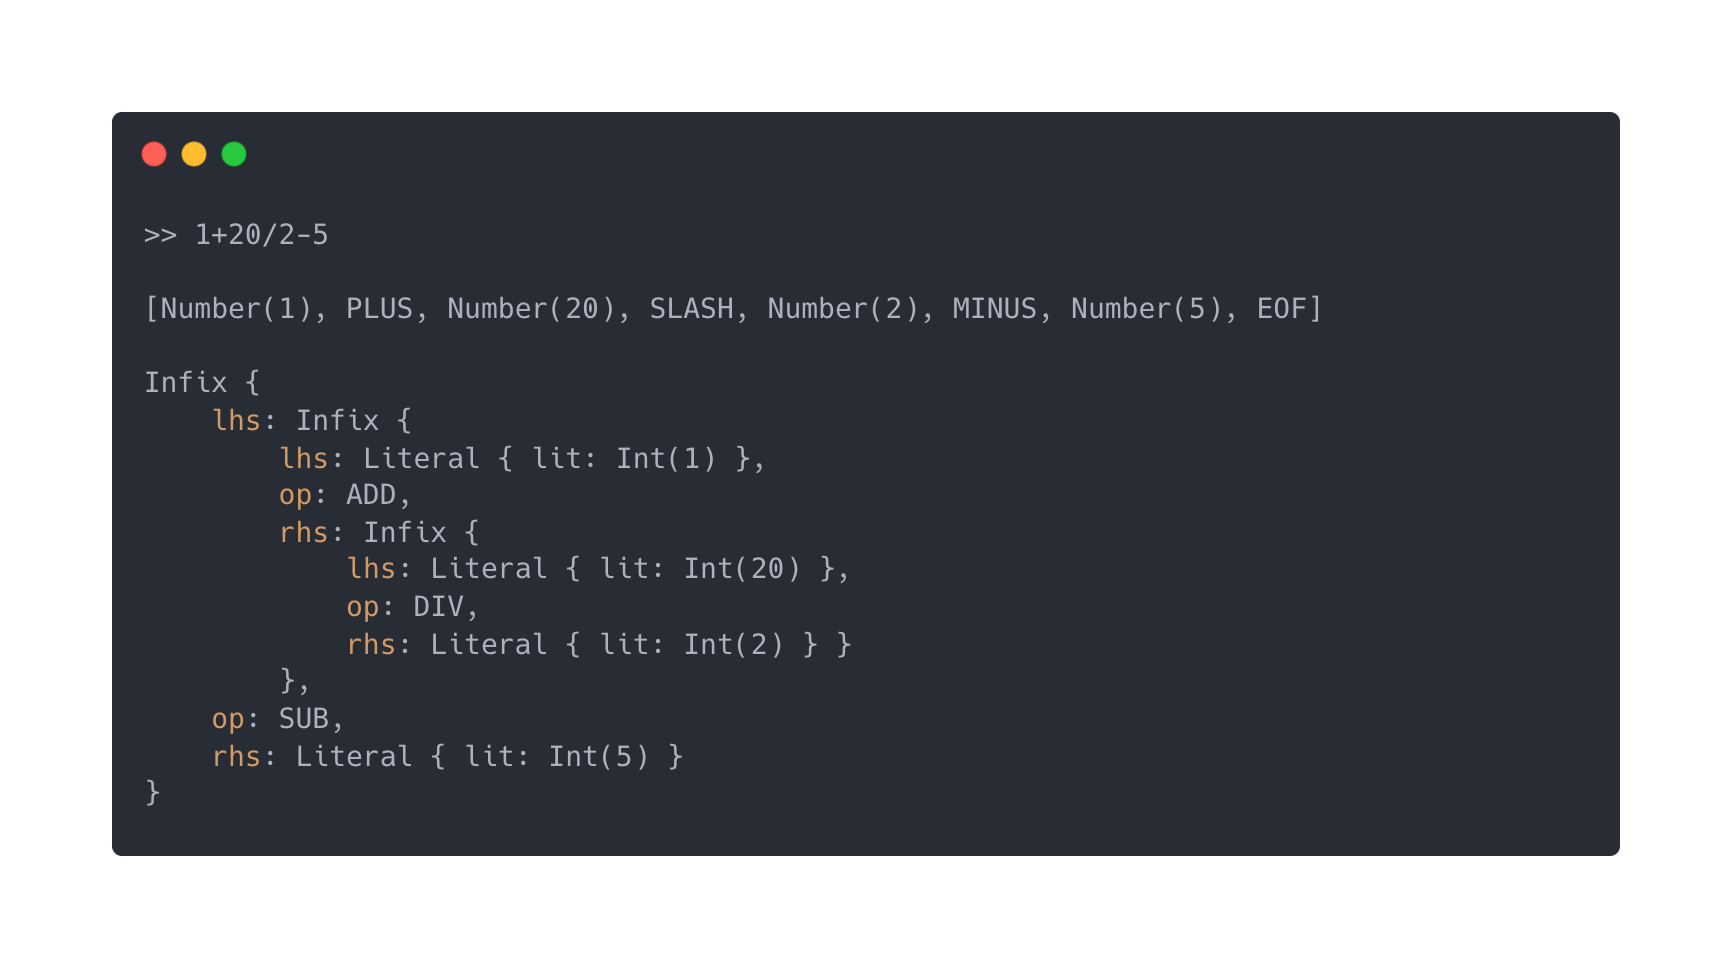
\includegraphics[width=12cm]{1. Unit Test.png}}
        & 
        The expected tokens are output by the lexer, and the parser produces an AST which correctly represents the order of operations in the given expression, indicating the pratt parser is working correctly. 
        \\
    \hline
        \raisebox{-\totalheight}{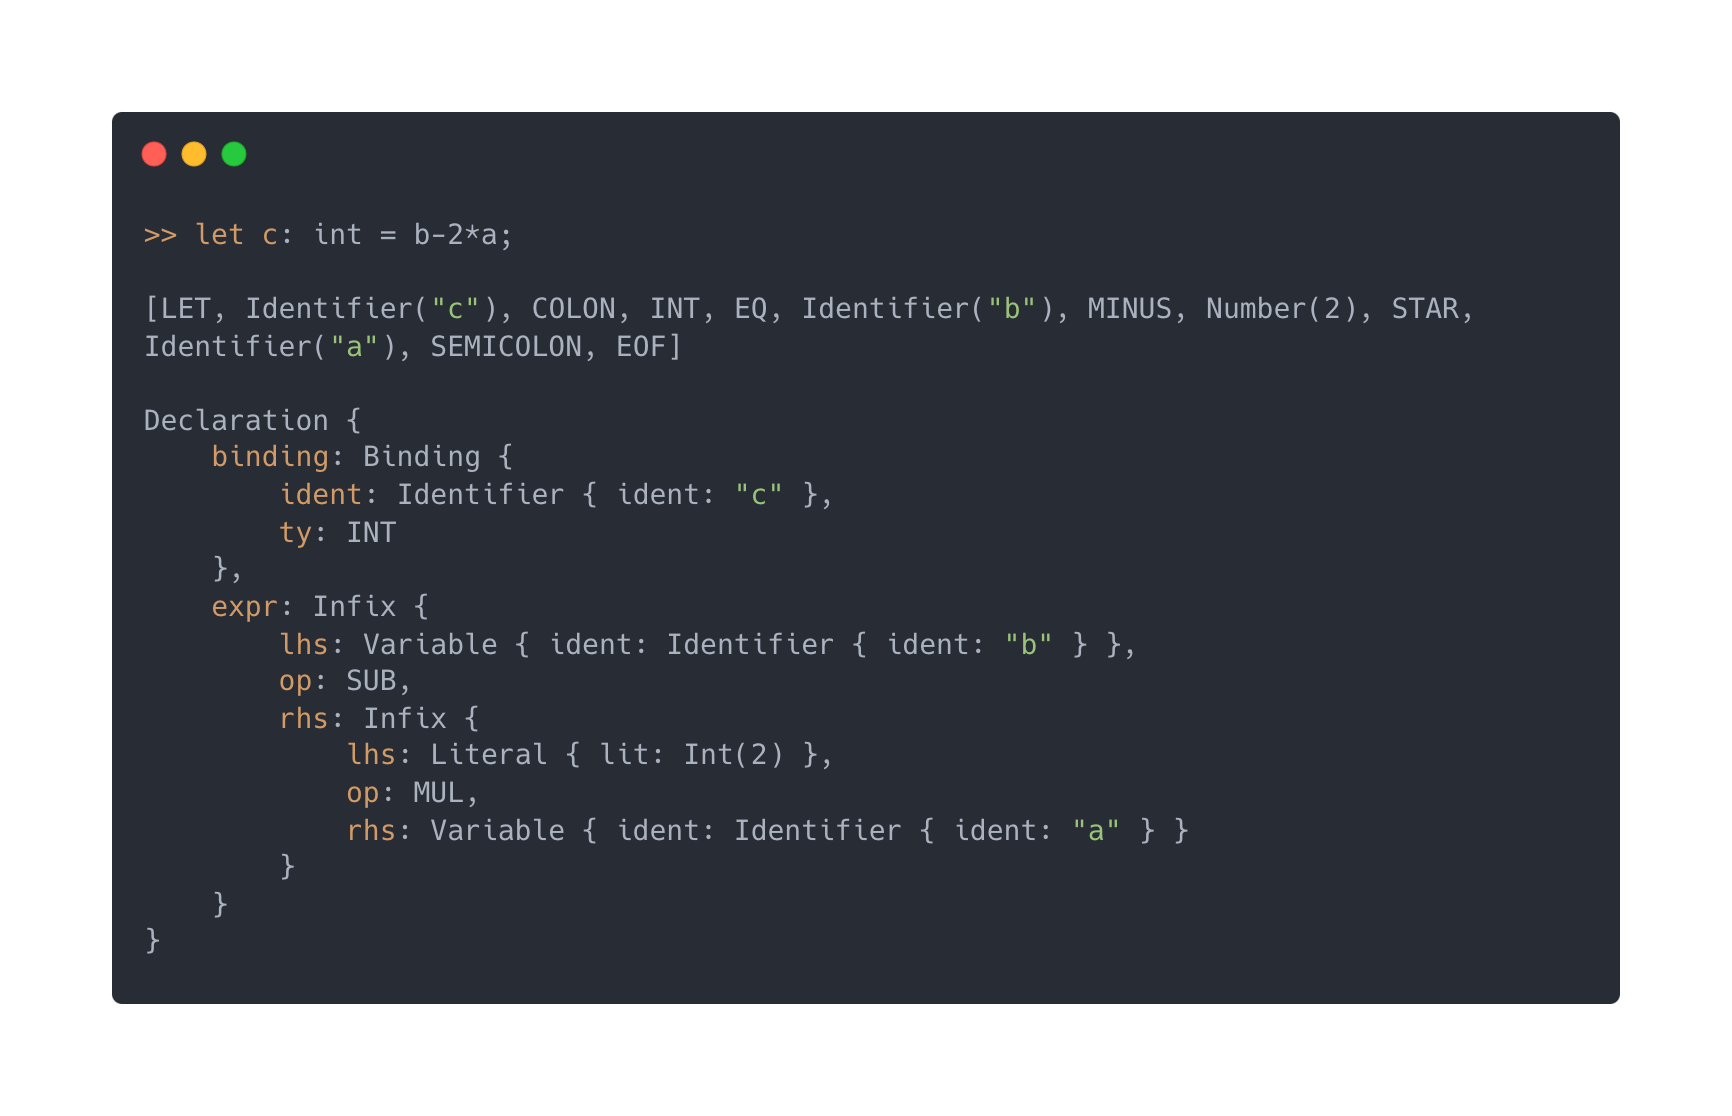
\includegraphics[width=12cm]{2. Unit Test.png}}
        & 
        The correct data-type has been parsed for the declaration binding, and the order of operations of the 'rhs' expression of the assignment has been parsed correctly showing that this test case has passed. 
        \\
    \hline
        \raisebox{-\totalheight}{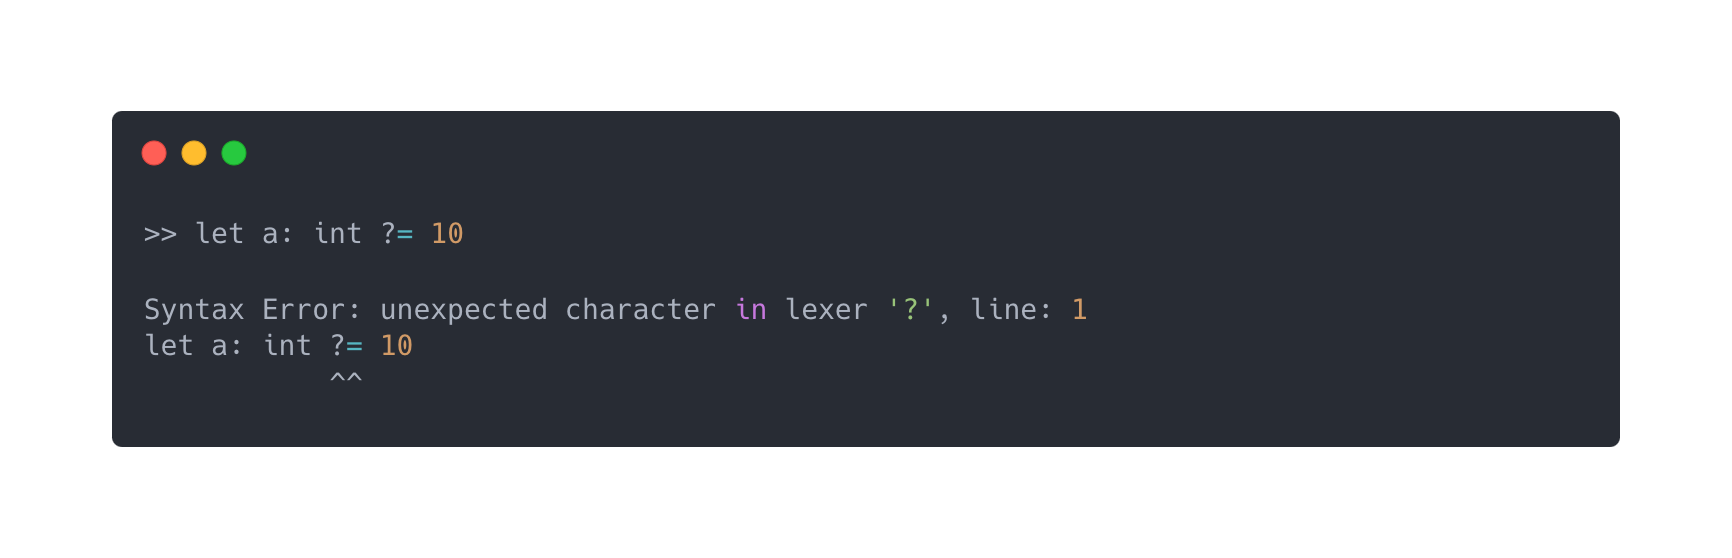
\includegraphics[width=12cm]{3. Unit Test.png}}
        & 
        The lexer successfully threw a syntax error when it encountered an unexpected character in the source code, pointing to the specific location in the error message and passing this test.
        \\
    \hline
        \raisebox{-\totalheight}{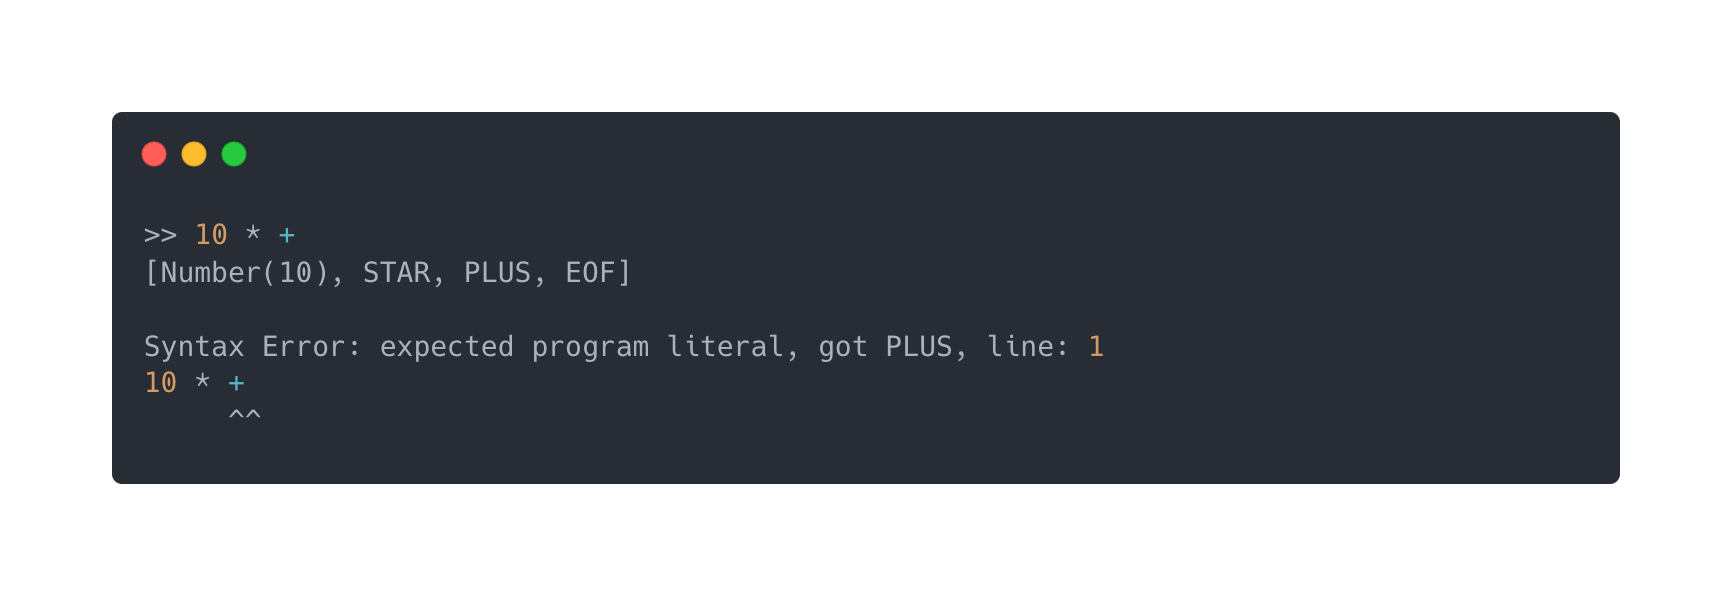
\includegraphics[width=12cm]{4. Unit Test.png}}
        & 
        The pratt parser determined the expression was invalid when it encountered an unexpected token (another operator). It successfully halted compilation and threw the correct error message, passing the test. 
        \\
    \hline
        \raisebox{-\totalheight}{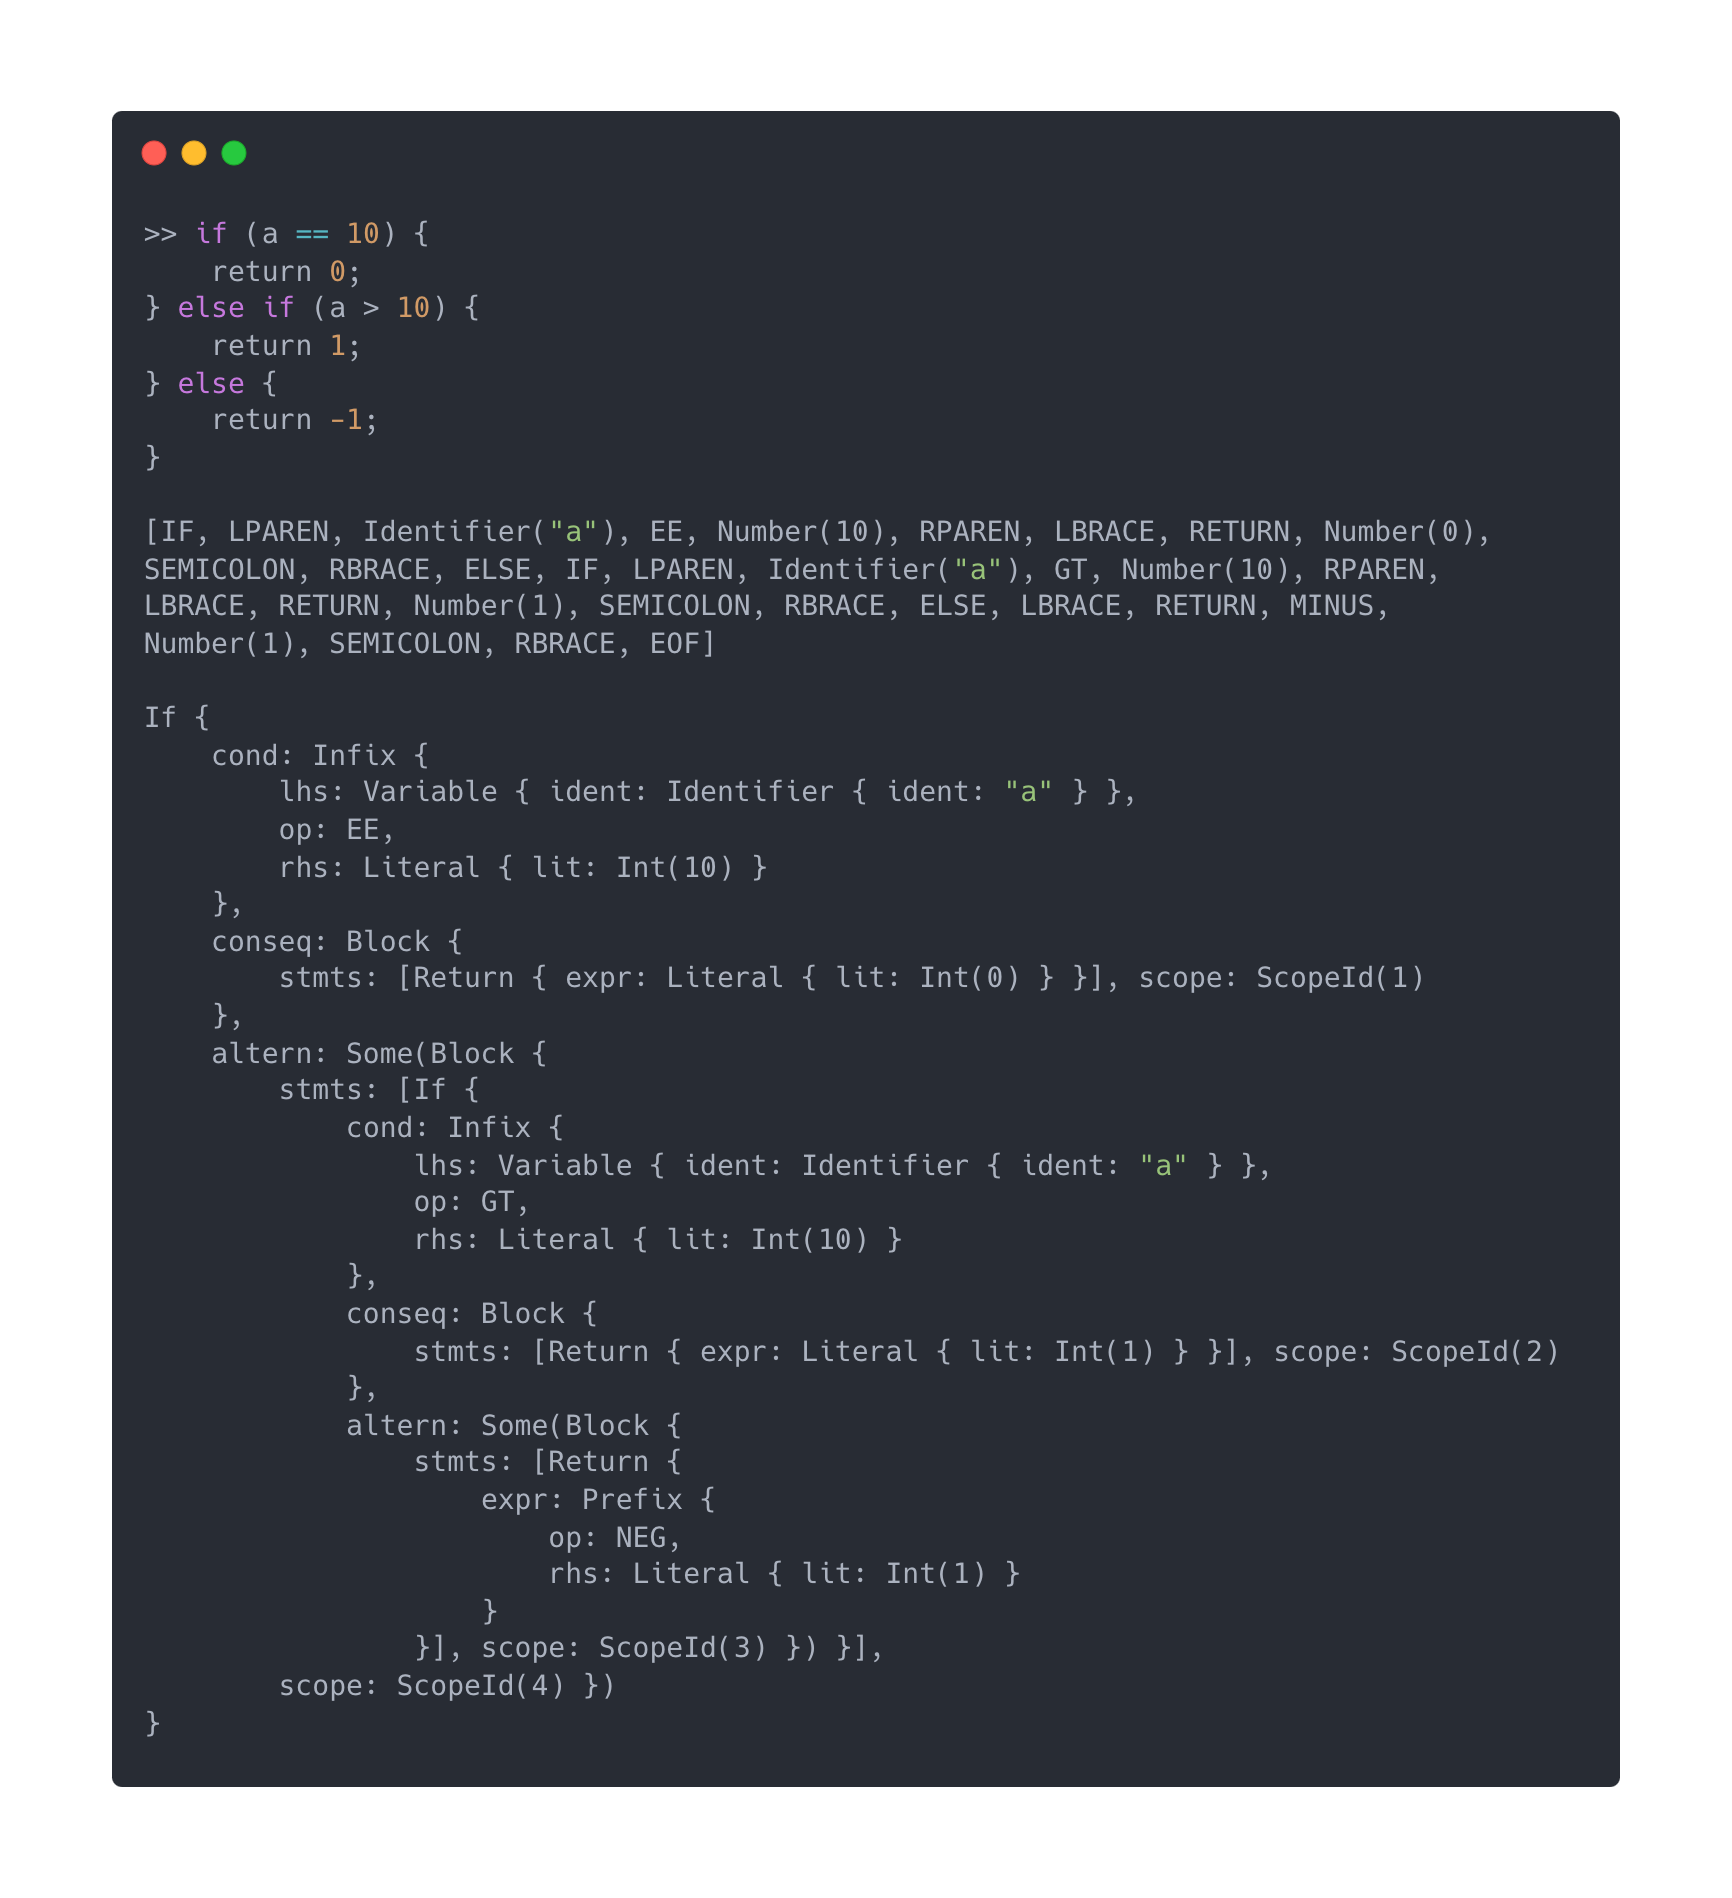
\includegraphics[width=12cm]{5. Unit Test.png}}
        & 
        The lexer produced the expected tokens from the source code, and the parser correctly represented the if statements in the abstract syntax tree, passing the test. The 'else if' clause was interpreted as the 'altern' attribute in the top-level if statement, with the 'else' clause being the 'altern' field of the second level if satement, exhibiting the intended behaviour when parsing if-else if statements. Furthermoer each 'Block' node was assigned its own unique ScopeID which is used for referencing local variables. Finally, the last feature showing the parser passed this test was that '-1' was parsed as a Prefix node, rather than the parser attempting to interpret it as an infix expression and throwing an error. 
        \\
    \hline
        \raisebox{-\totalheight}{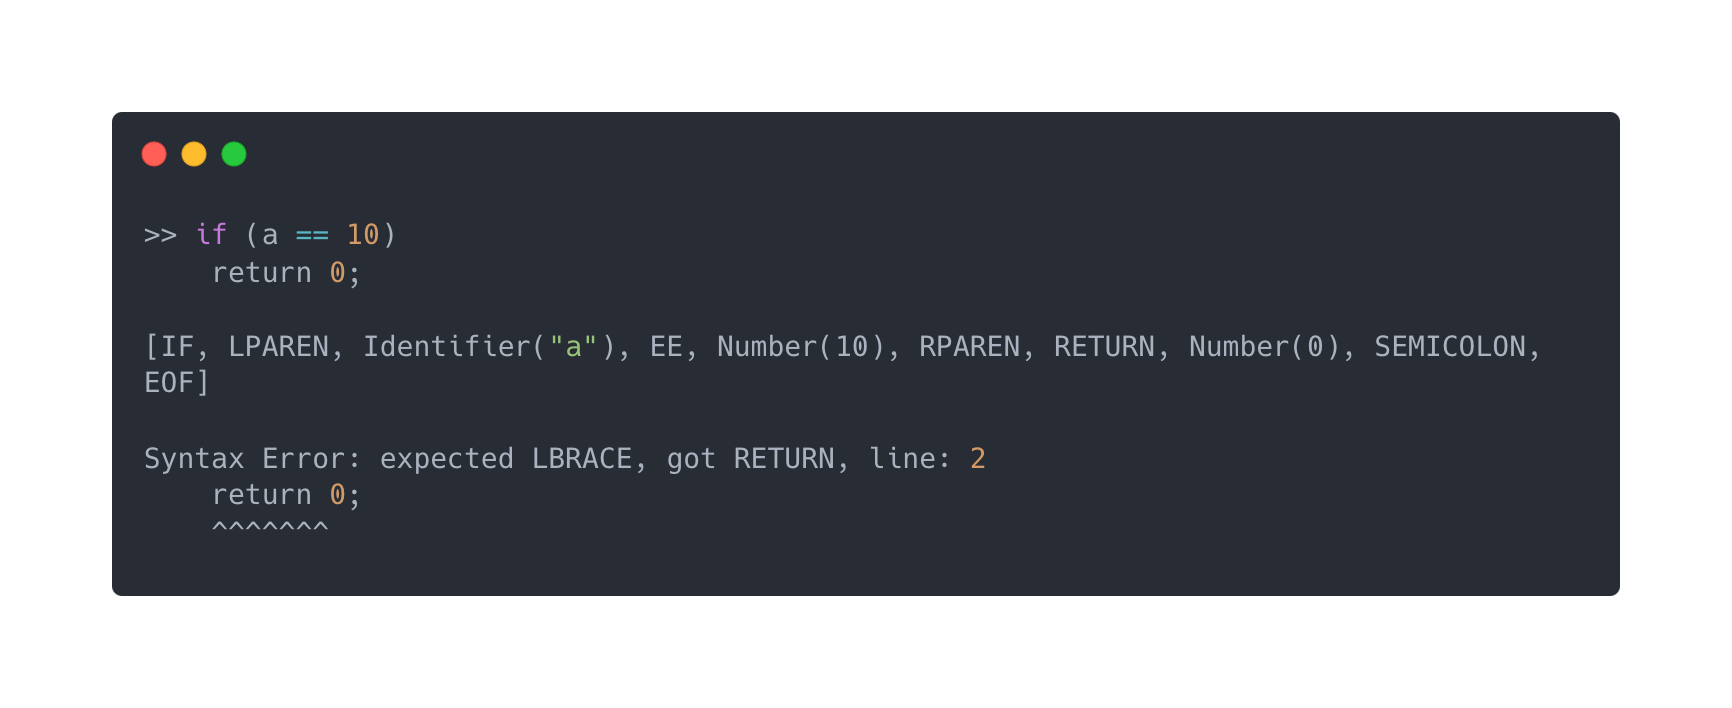
\includegraphics[width=12cm]{6. Unit Test.png}}
        & 
        When attempting to parse the if statement, the parser expects a '\{' token. When, instead it encounters the 'return' keyword - it throws a SyntaxError due to the missing character. This error successfully points to the position of the unexpected token, passing the test.
        \\
    \hline
        \raisebox{-\totalheight}{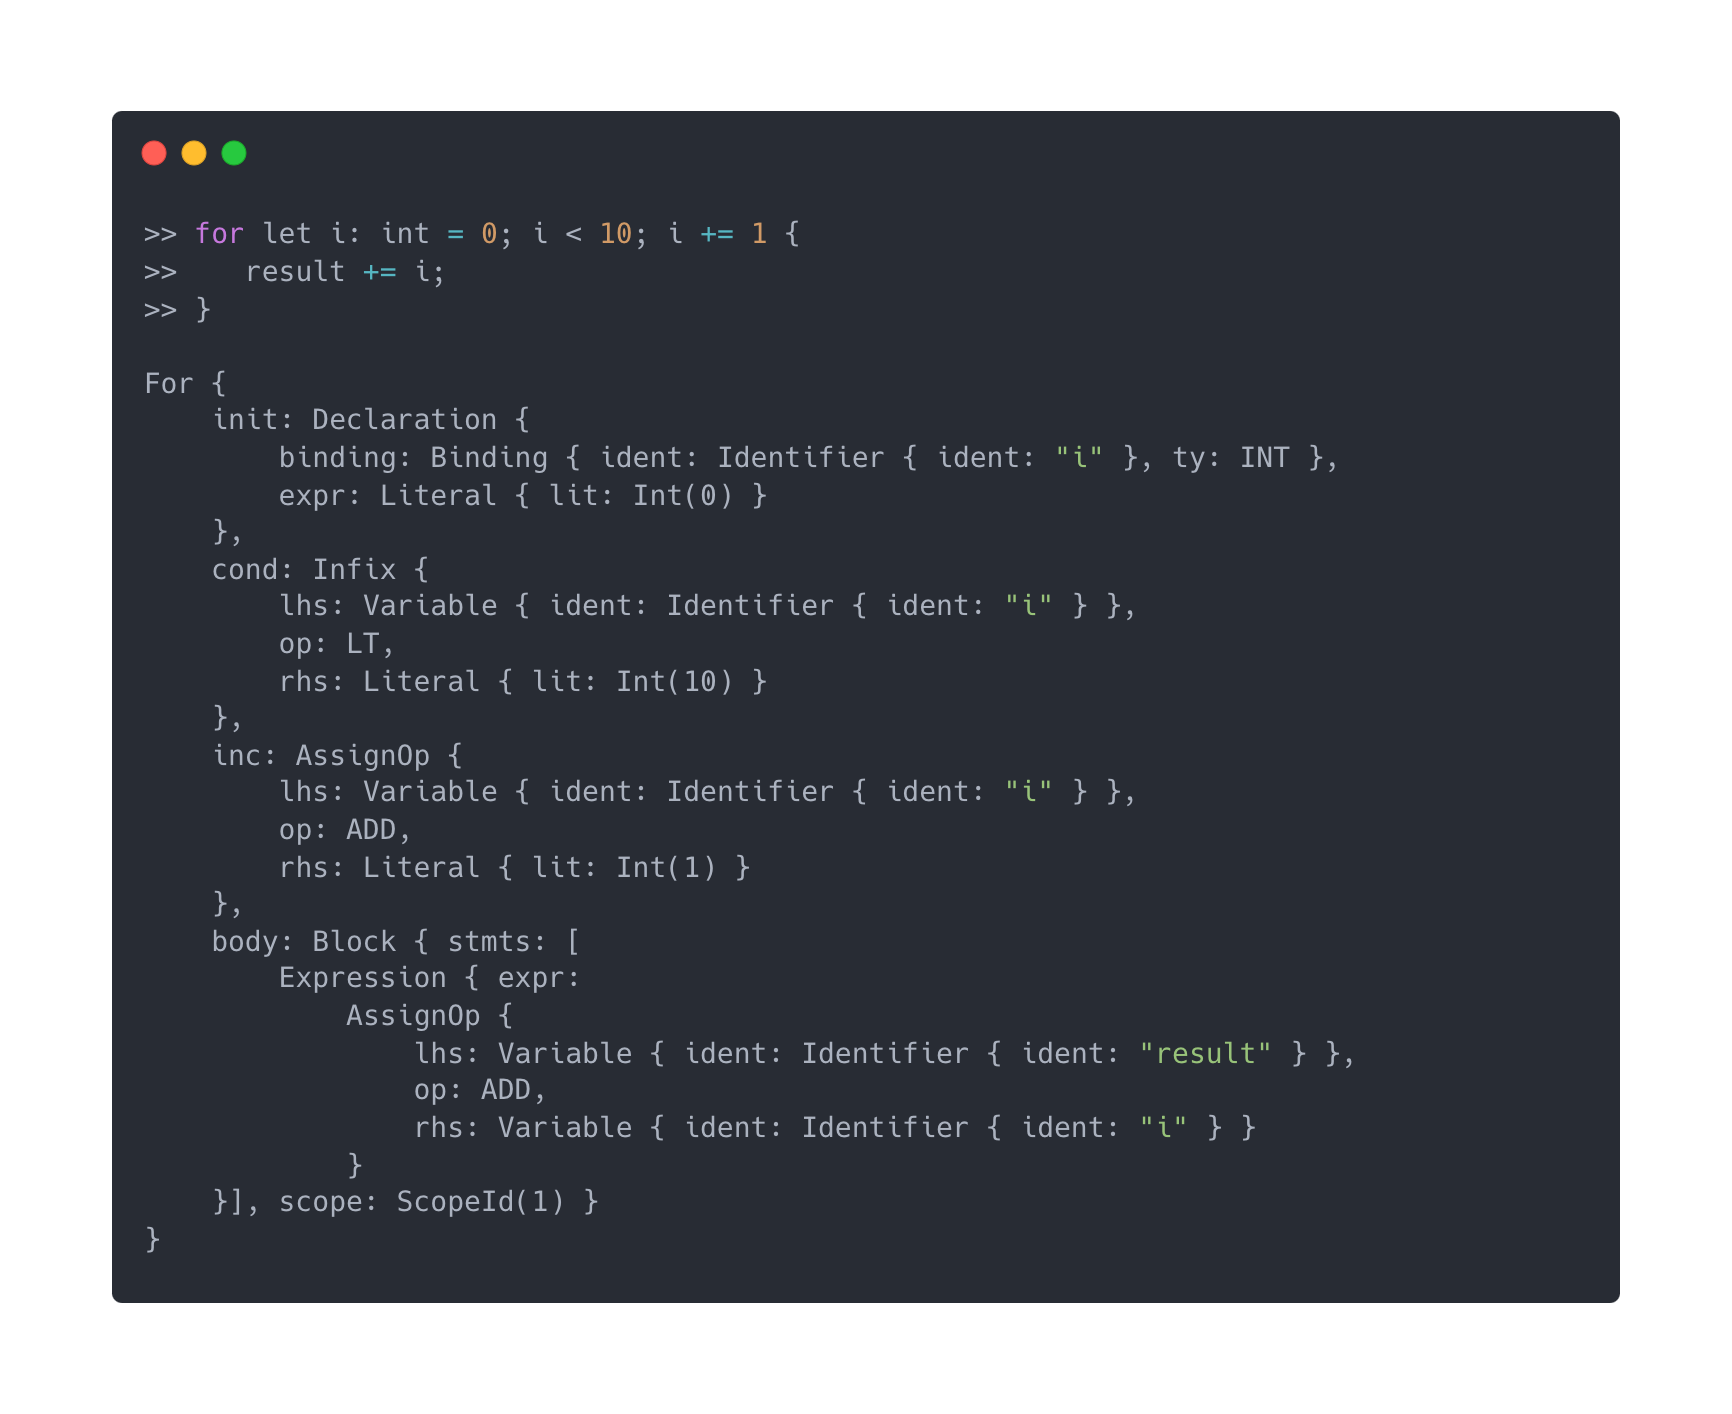
\includegraphics[width=12cm]{8. Unit Test.png}}
        & 
        The parser assigns the correct expressions to the initialise, condition and increment fields of the for loop. Noting that whilst the initialise field is supposed to be a STATEMENT type, the other two are both EXPRESSIONs. The '+=' increment-assign operation is successfully parsed as a 'PLUS' OPERATOR and stored as an EXPRESSION in the increment field, matching the expected result for this test.  
        \\
    \hline
        \raisebox{-\totalheight}{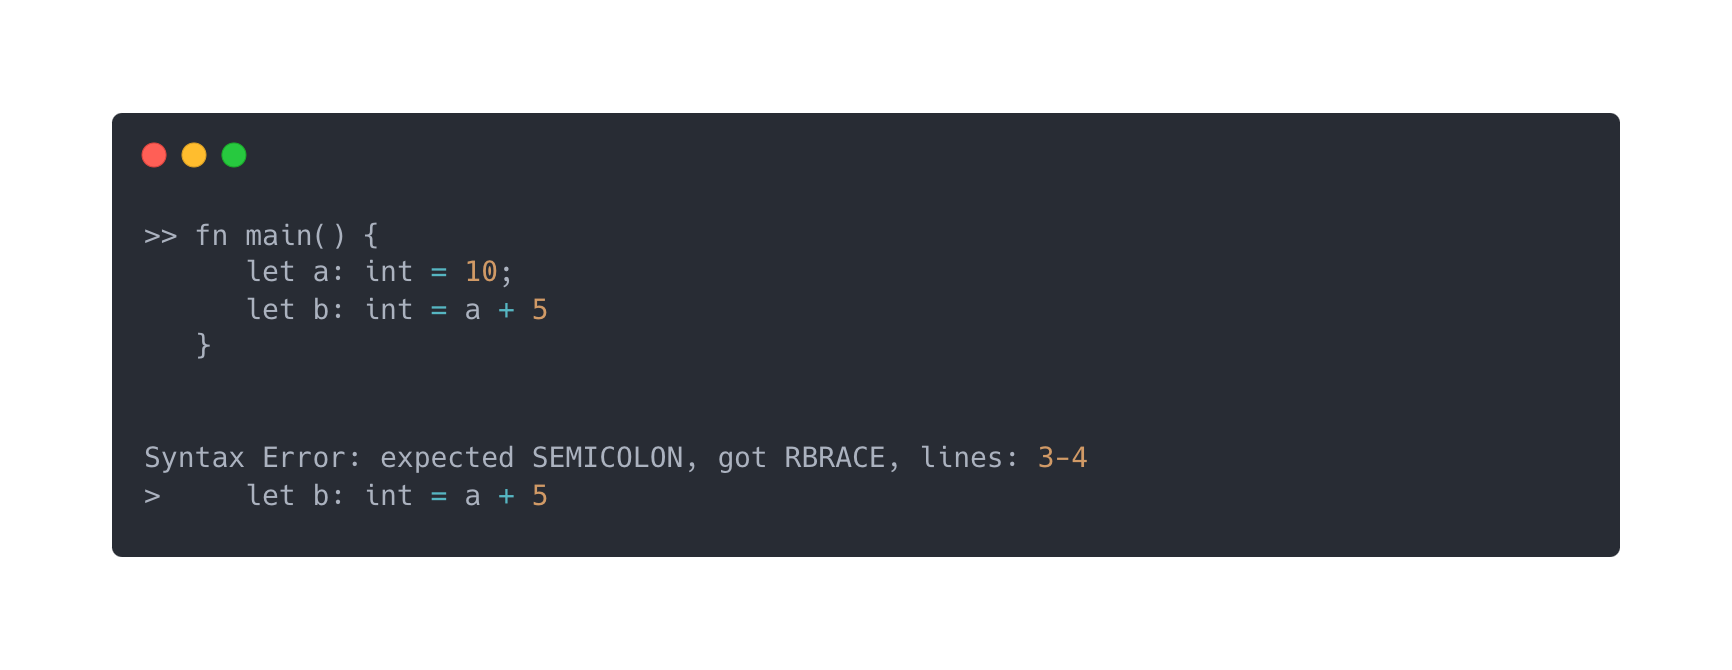
\includegraphics[width=12cm]{14. Unit Test.png}}
        & 
        When parsing the source code, the parser notices that line 3 isn't terminated by a semicolon. It successfully throws a SyntaxError and points out the location of this error in source code, passing this test. 
        \\
    \hline
\end{longtable}

\subsubsection{Semantic Analysis}

The second set of algorithms I want to test is the Sentiment Analysis phase of the compiler. Once a valid program is parsed into an abstract syntax tree, the AST is checked for further errors including references to undeclared variables or subroutines, and expressions where the data types are not compatible. Furthermore, this phase is responsible for executing the constant folding algorithm. Each test case contains the program being compiled, followed by the output of the compiler (and potentially any intermediate steps). 

\begin{longtable}{|p{12cm}|p{4cm}|} 
    \hline
        Program & Result \\ 
    \hline
        \raisebox{-\totalheight}{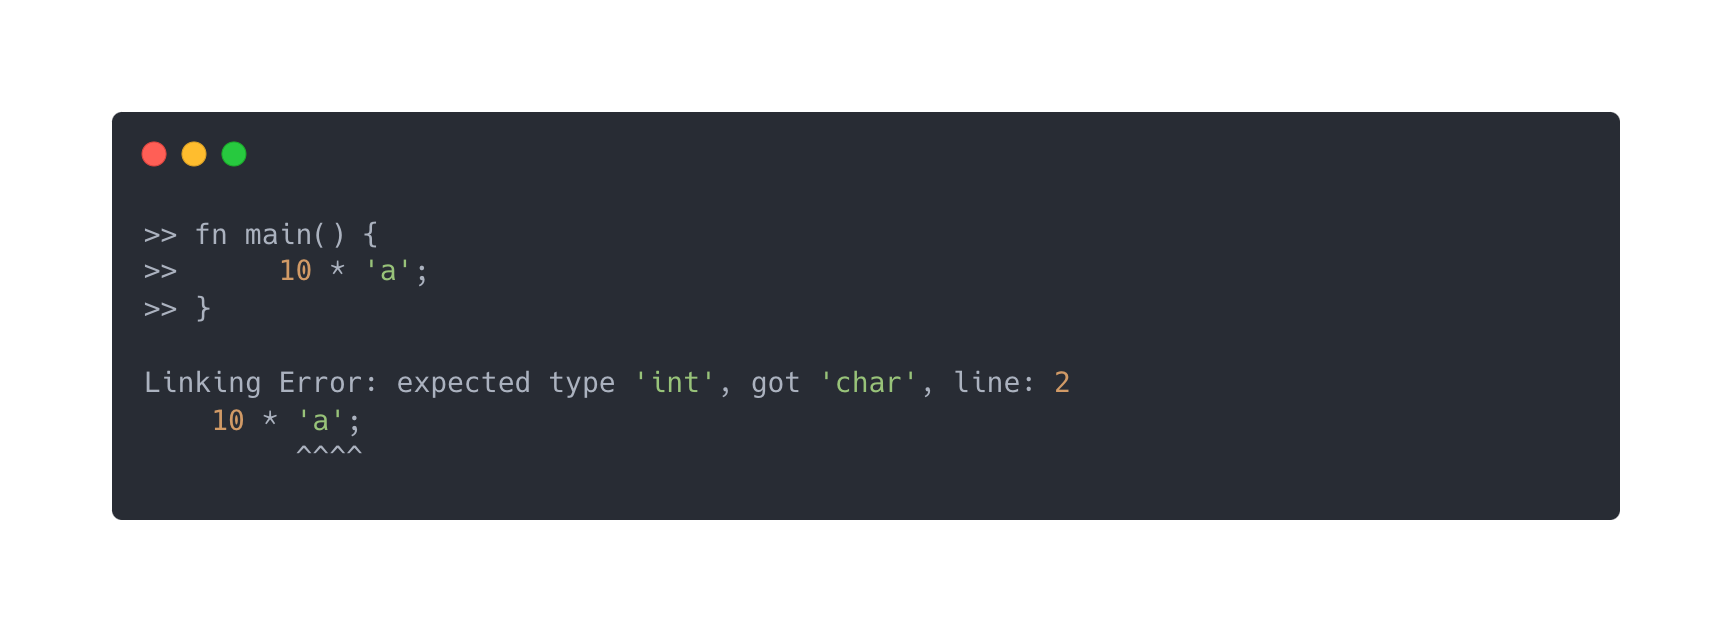
\includegraphics[width=12cm]{7. Unit Test.png}}
        & 
        After parsing the program, the AST is fed into the type checker. The type checker notices that a multiply operation is being performed on a character and an integer, two data types which are not compatible - and throws the correponding type error. Passing this test. 
        \\
    \hline
        \raisebox{-\totalheight}{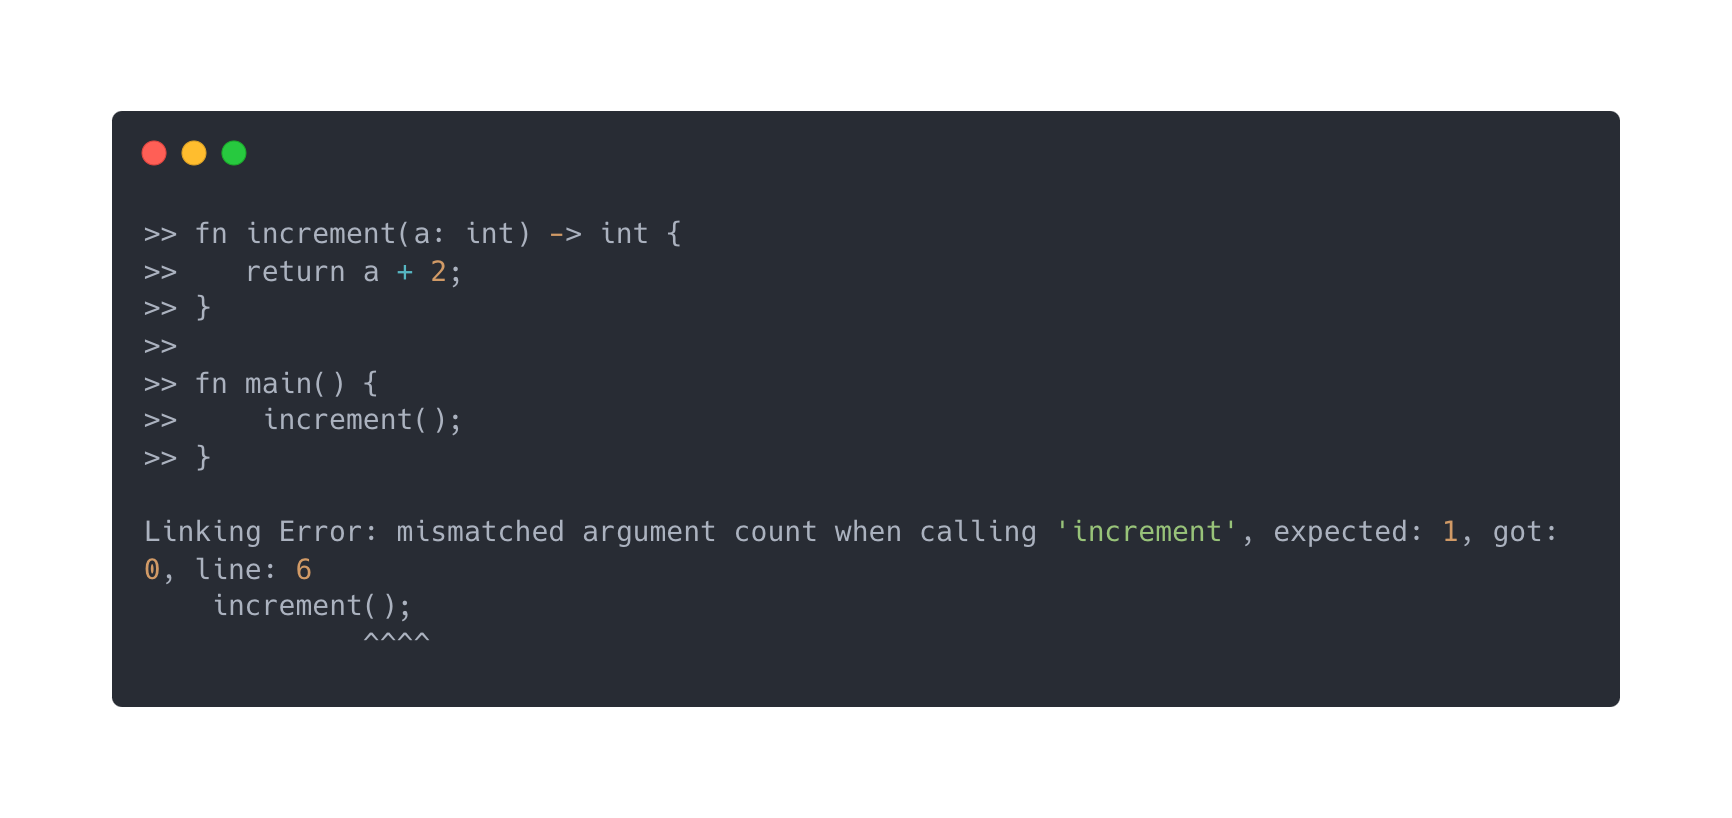
\includegraphics[width=12cm]{9. Unit Test.png}}
        & 
        The type checker is also responsible for validating the arguments passed to a function call. The testing video demonstrates when a function is called with an argument of an incorrect type, however this test demonstrates when a function is called with the incorrect number of arguments. The type checker compares the arguments passed in the function call to the parameter bindings specified in the function's definition - after noticing there is a mismatch, the type checker halts compilation and throws the correct error, pointing out the location of the invalid call in source code.
        \\
    \hline
        \raisebox{-\totalheight}{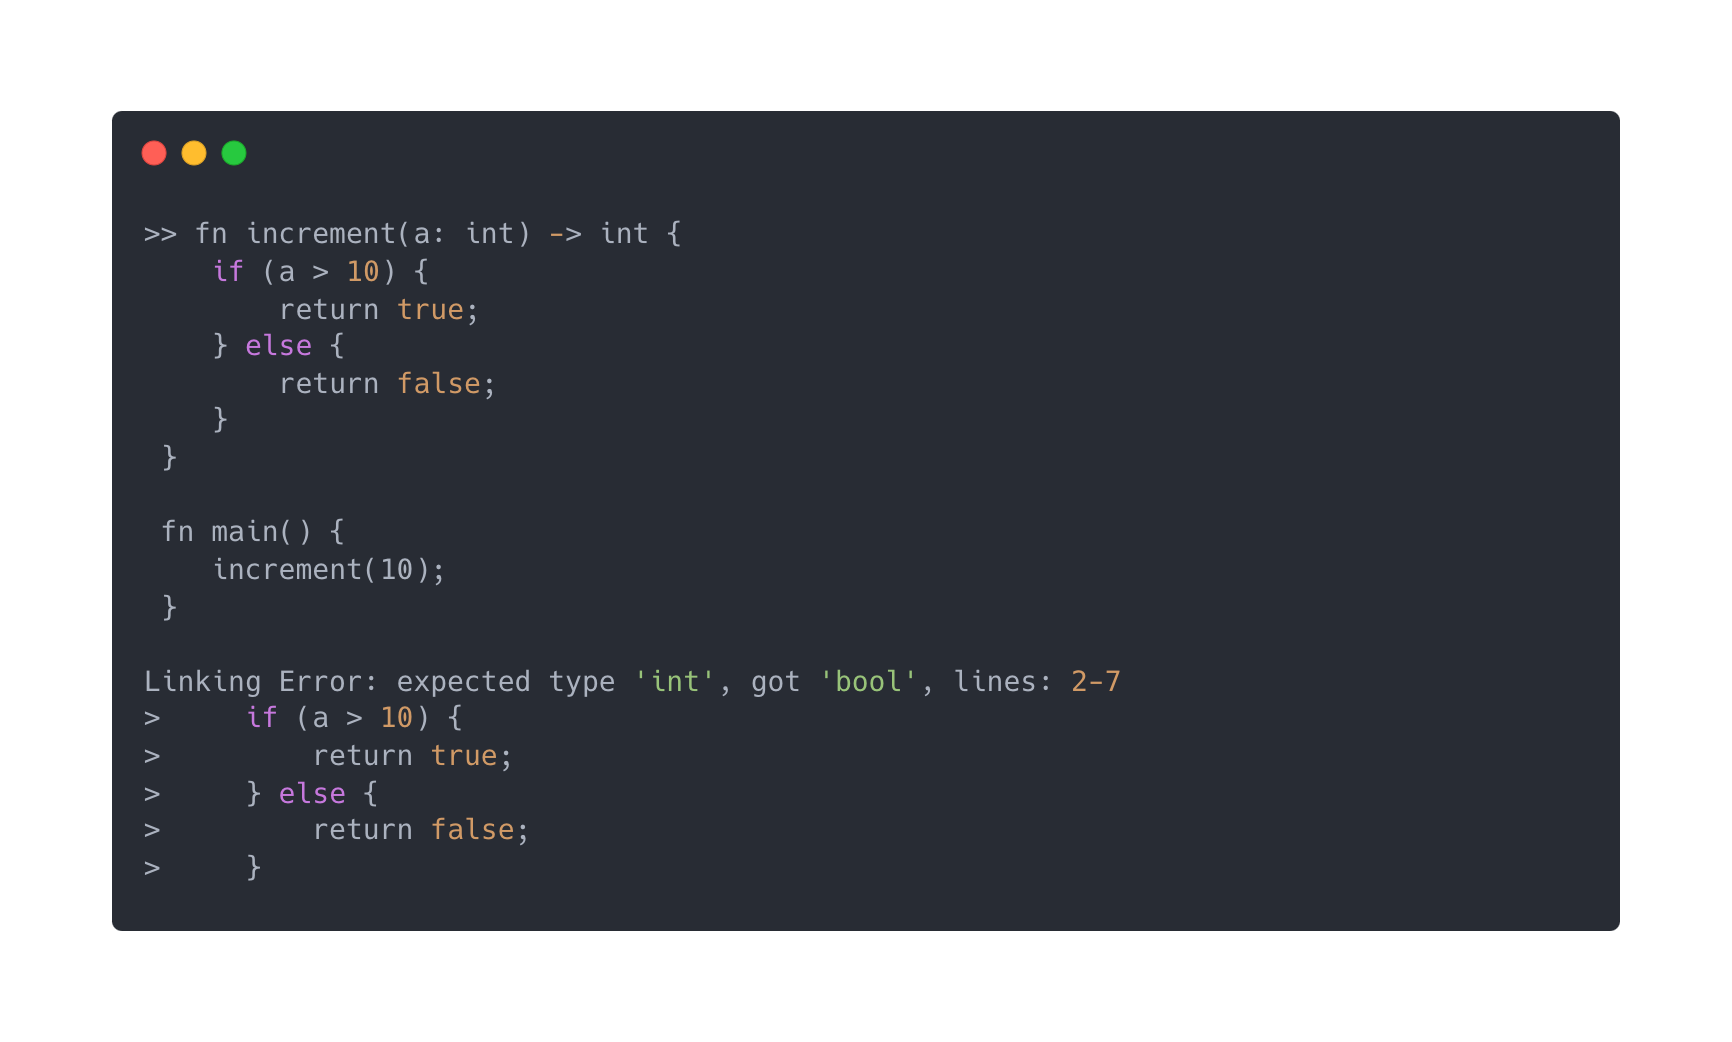
\includegraphics[width=12cm]{10. Unit Test.png}}
        & 
        This test validates that the type checker notices when a function is attempting to return a value of an unexpected type, even when that function contains multiple return points inside a conditional expression. The type checker notices that the return values are both booleans, however the function definition expects an integer to be returned. The type checker halts compilation and throws an error, pointing out the entire conditional statement as the location of the error, passing this test. 
        \\
    \hline
        \raisebox{-\totalheight}{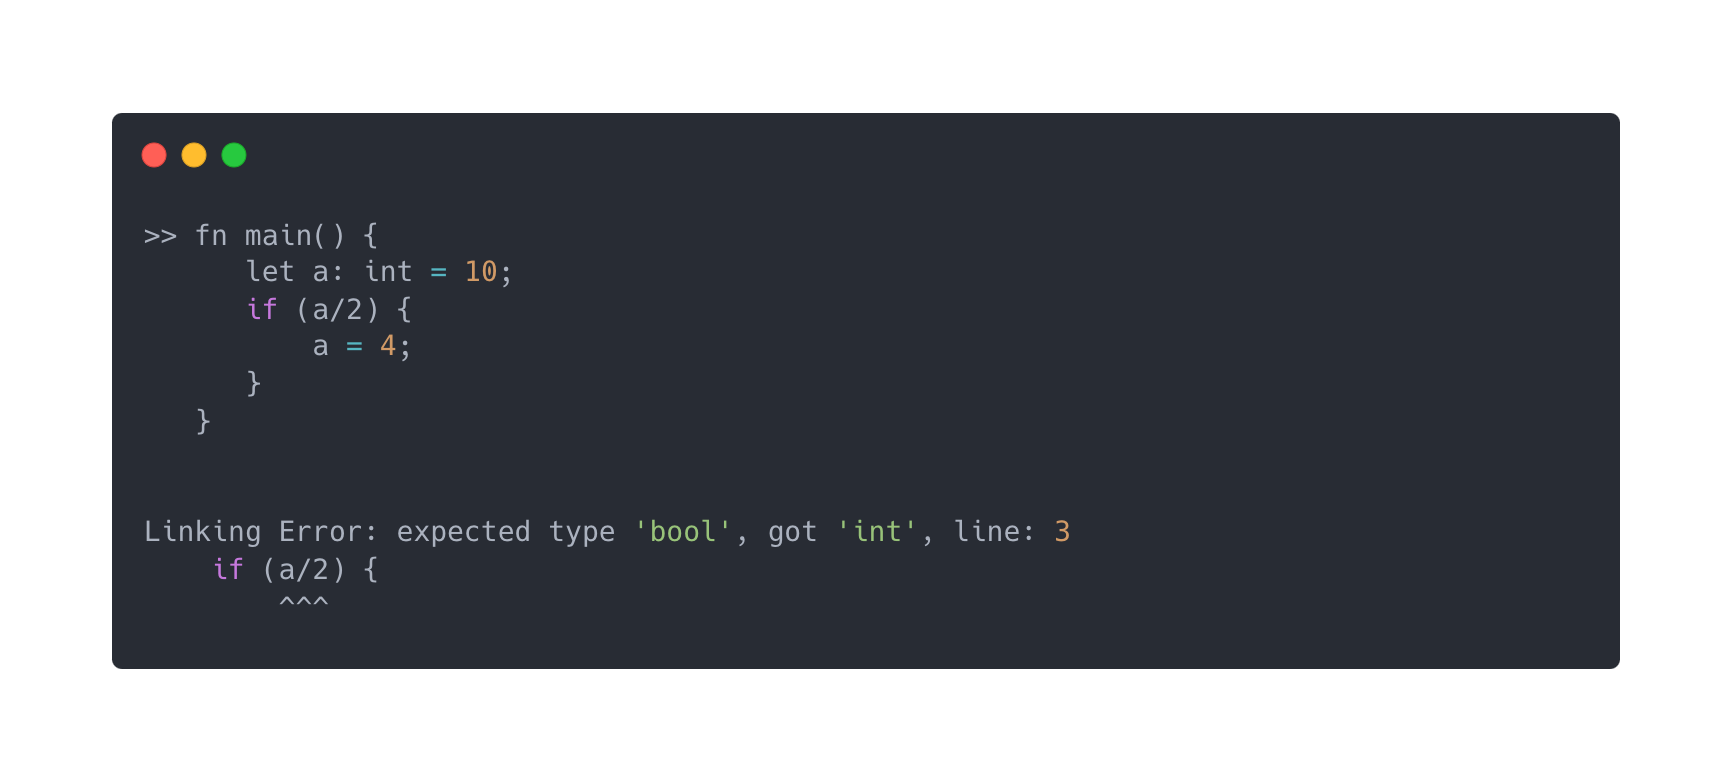
\includegraphics[width=12cm]{11. Unit Test.png}}
        & 
        The type checker determines that the expression inside the if node's condition will evaluate to an integer and since if-nodes require their conditionals to operate on boolean values, the type checker throws an error, pointing to the location of the expression in source code. Passing this test. 
        \\
    \hline
        \raisebox{-\totalheight}{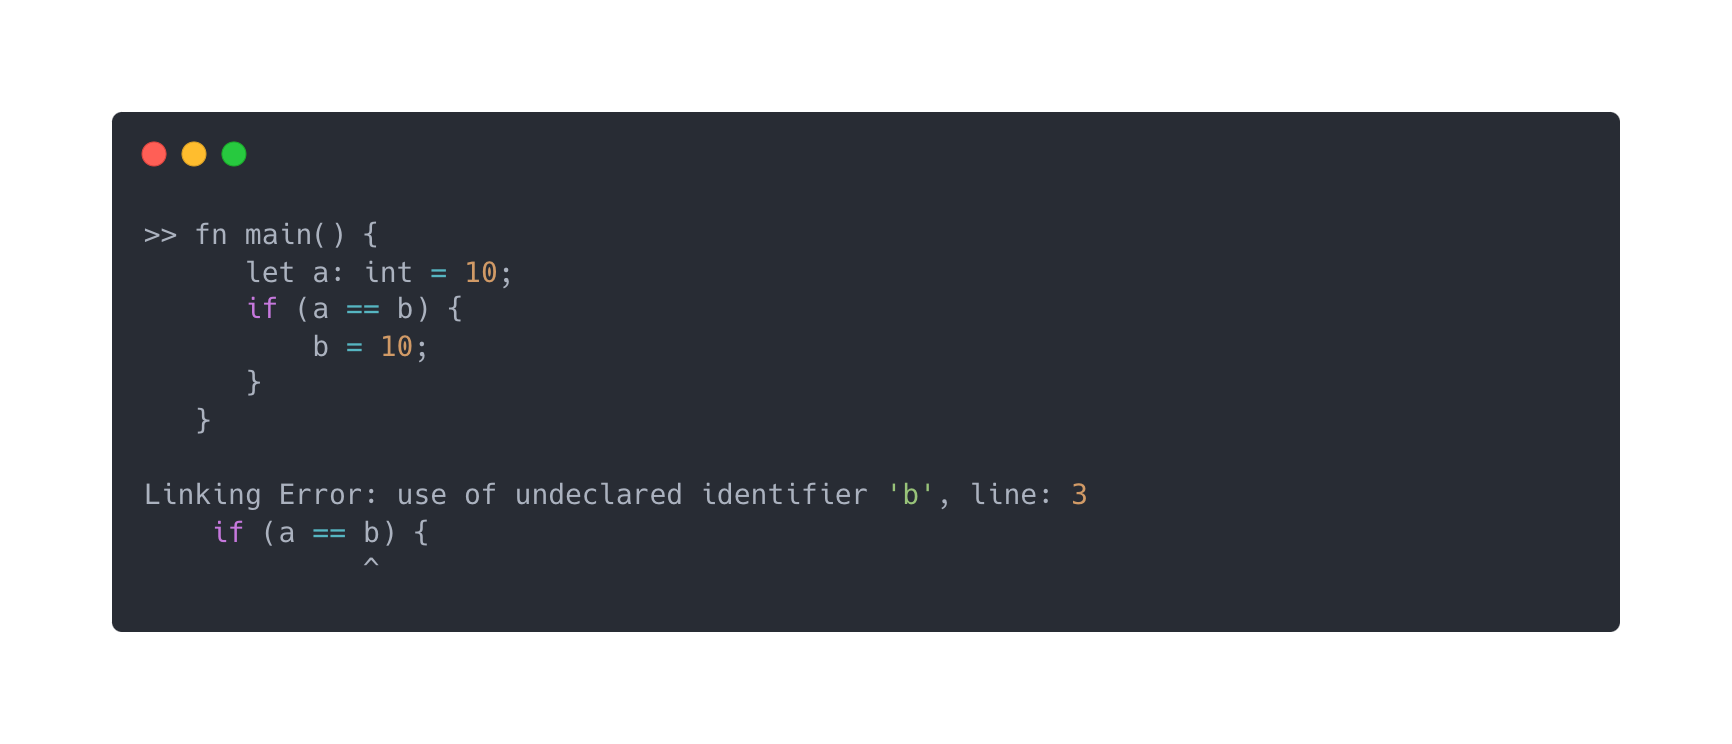
\includegraphics[width=12cm]{12. Unit Test.png}}
        & 
        When building up the scope table during sentiment analysis, it notices that the variable 'b' hasn't been declared before it was used in the program. The scope table builder then successfully throws an error and halts compilation. 
        \\
    \hline
        \raisebox{-\totalheight}{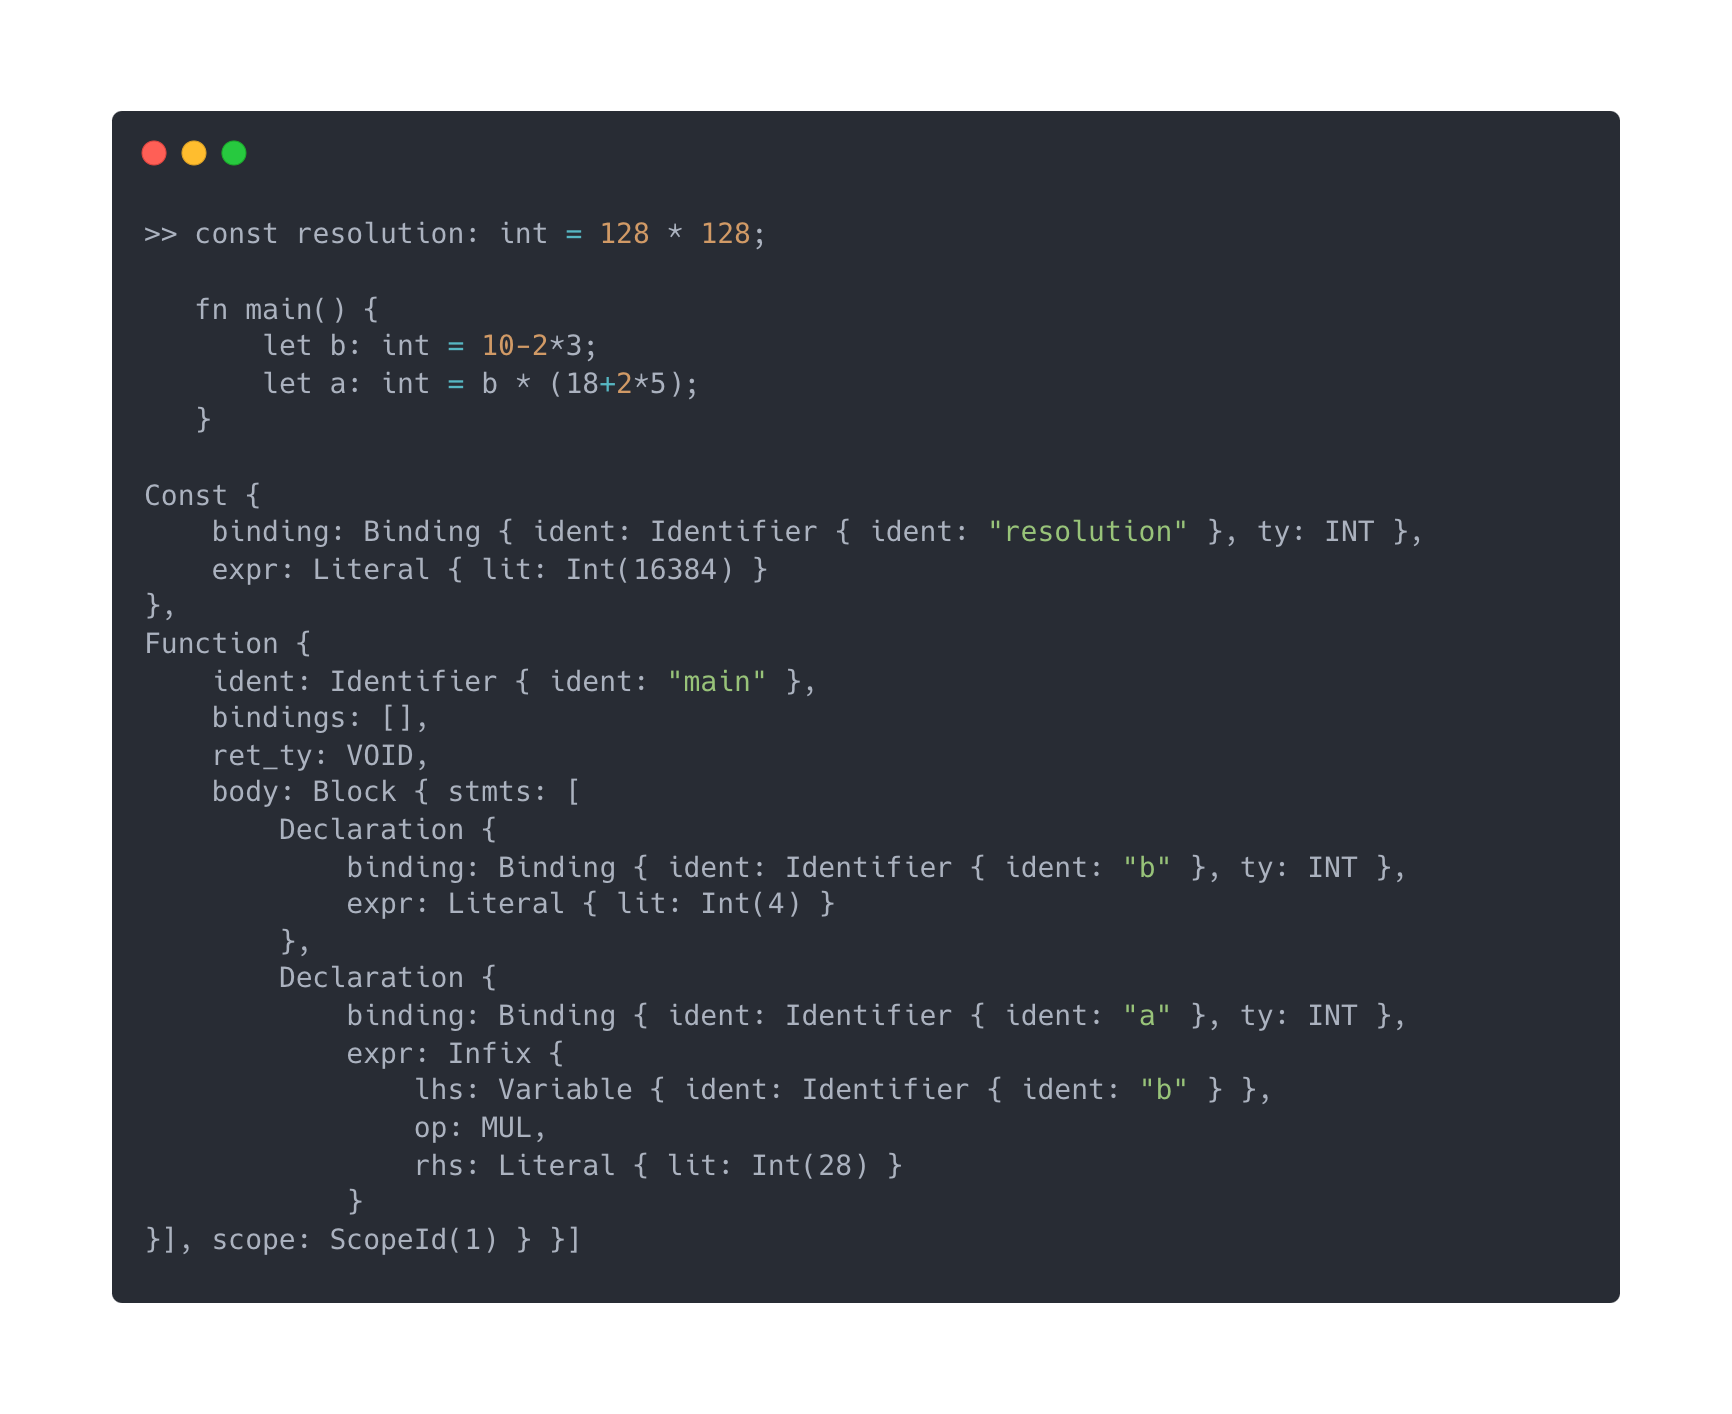
\includegraphics[width=12cm]{13. Unit Test.png}}
        & 
        This test case validates constant folding within the compiler. The compiler successfully noticed that the expressions '128*128', '10-2*3', and '18+2*5' could be evaluated to integers since they contain no references to variables, and replaces the entire expression with a single literal node containing its evaluated result. The expression '18+2*5' forms part of the larger expression 'b * (18+2*5)'. The algorithm is able to isolate the part of this expression that can be evaluated into an integer, and correctly replaces the expression with 'b*28'. Passing this test.
        \\
    \hline
\end{longtable}